    % This file is part of nrf_seminar.

    % nrf_seminar is free software: you can redistribute it and/or modify
    % it under the terms of the GNU General Public License as published by
    % the Free Software Foundation, either version 3 of the License, or
    % (at your option) any later version.

    % nrf_seminar is distributed in the hope that it will be useful,
    % but WITHOUT ANY WARRANTY; without even the implied warranty of
    % MERCHANTABILITY or FITNESS FOR A PARTICULAR PURPOSE.  See the
    % GNU General Public License for more details.

    % You should have received a copy of the GNU General Public License
    % along with nrf_seminar.  If not, see <https://www.gnu.org/licenses/>.

\begin{textblock}{9.5}(0., -4.)
    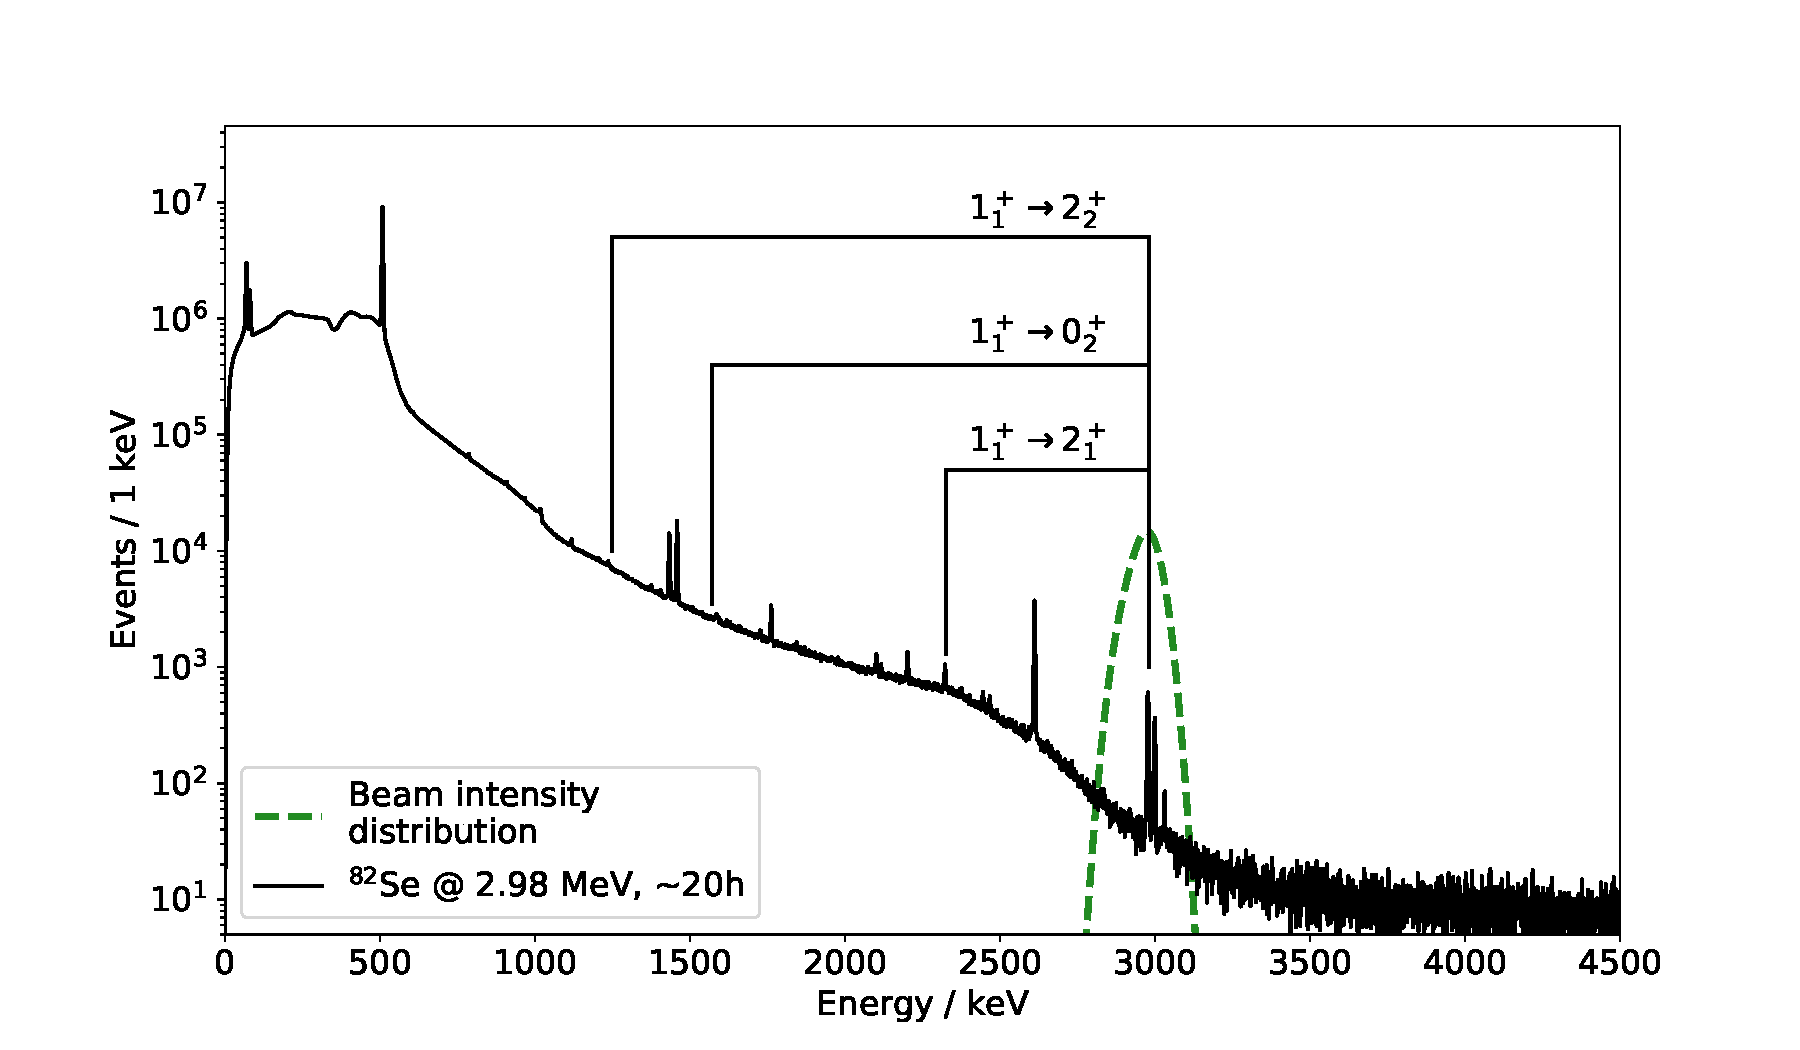
\includegraphics[width=\textwidth, trim=50 0 50 50,clip]{figures/se82_spectrum_branchings.pdf}
\end{textblock}

\begin{textblock}{5.}(10., -5)
    \color{green}\textbf{Advantages} \color{black} of the NRF technique
    \begin{itemize}
        \item Model-independent
        \item High resolution
        \item (Selectivity)
    \end{itemize}
    
    \color{red}\textbf{Disadvantages}\color{black}
    \begin{itemize}
        \item Nonresonant background
        \item Low cross section (long experiments, large samples, stable isotopes)
        \item Inefficient detection
    \end{itemize}
\end{textblock}